
\documentclass[DIV=calc, paper=letter, fontsize=11pt]{scrartcl}	 % A4 paper and 11pt font size

\usepackage[body={6.5in,9.0in},
  top=1.0in, left=1.0in]{geometry}
  
\usepackage[english]{babel} % English language/hyphenation
\usepackage[protrusion=true,expansion=true]{microtype} % Better typography
\usepackage{amsmath,amsfonts,amsthm} % Math packages
\usepackage[svgnames]{xcolor} % Enabling colors by their 'svgnames'
\usepackage[hang, small,labelfont=bf,up,textfont=it,up]{caption} % Custom captions under/above floats in tables or figures
\usepackage{booktabs} % Horizontal rules in tables
\usepackage{fix-cm}	 % Custom font sizes - used for the initial letter in the document
\usepackage{epsfig}
\usepackage{sectsty} % Enables custom section titles
\allsectionsfont{\usefont{OT1}{phv}{b}{n}} % Change the font of all section commands

\usepackage{fancyhdr} % Needed to define custom headers/footers
\pagestyle{fancy} % Enables the custom headers/footers
\usepackage{lastpage} % Used to determine the number of pages in the document (for "Page X of Total")
\usepackage{color}

\usepackage{fancyvrb}% used to include files verbatim
%\usepackage{chemsym}

\usepackage{hyperref}

\usepackage[backend=bibtex,style=numeric,sorting=ydnt,maxnames=15]{biblatex}
\renewbibmacro{in:}{}

% Count total number of entries in each refsection
\AtDataInput{%
  \csnumgdef{entrycount:\therefsection}{%
    \csuse{entrycount:\therefsection}+1}}

% Print the labelnumber as the total number of entries in the
% current refsection, minus the actual labelnumber, plus one
\DeclareFieldFormat{labelnumber}{\mkbibdesc{#1}}    
\newrobustcmd*{\mkbibdesc}[1]{%
  \number\numexpr\csuse{entrycount:\therefsection}+1-#1\relax}


%\addbibresource[label=papers]{mypubs.bib}
%\addbibresource[label=books]{mypubs.bib}
%\addbibresource[label=edited]{mypubs.bib}
%\addbibresource[label=chapters]{mypubs.bib}


% Headers - all currently empty
\lhead{}
\chead{}
\rhead{}

% Footers
\lfoot{\textsf{EBSD/ECP} manual, v3.0, \today}
\cfoot{}
\rfoot{\footnotesize Page \thepage\ of \pageref{LastPage}} % "Page 1 of 2"

\renewcommand{\headrulewidth}{0.0pt} % No header rule
\renewcommand{\footrulewidth}{0.4pt} % Thin footer rule

\usepackage{lettrine} % Package to accentuate the first letter of the text
\newcommand{\initial}[1]{ % Defines the command and style for the first letter
\lettrine[lines=3,lhang=0.3,nindent=0em]{
\color{DarkGoldenrod}
{\textsf{#1}}}{}}

\usepackage{titling} % Allows custom title configuration

\newcommand{\HorRule}{\color{DarkGoldenrod} \rule{\linewidth}{1pt}} % Defines the gold horizontal rule around the title

\pretitle{\vspace{-1.5in} \begin{center} \HorRule \fontsize{25}{25} \usefont{OT1}{phv}{b}{n} \color{DarkRed} \selectfont} % Horizontal rule before the title

\title{EMSoft\\ EBSD, ECP and Kossel Simulations} % Your article title

\posttitle{\par\end{center}\vskip 0.5em} % Whitespace under the title

\preauthor{\begin{center}\large \lineskip 0.5em \usefont{OT1}{phv}{b}{sl} \color{DarkRed}} % Author font configuration

\author{\vspace*{-0.7in}} % Your name

\postauthor{\footnotesize \usefont{OT1}{phv}{m}{sl} \color{Black} % Configuration for the institution name

\par\end{center}\HorRule} % Horizontal rule after the title
\date{Program Manual, v3.0, \today\protect\footnote{This set of programs was developed with financial support from two agencies. 
The Office of Naval Research sponsored the development of the original version 2.0 f90 source code for computation of EBSD patterns in research 
grant N00014-12-1-0075.  The IDL visualization interface, and the complete version 3.0 (including ECP) and beyond were developed with financial 
support from an AFOSR/MURI grant FA9550-12-1-0458.}}

\newcommand{\ctp}{\textsf{EMSoft}}
%
\newcommand{\upg}[1]{\mathrm{i}U_{\mathbf{#1}}^{\prime}}
\newcommand{\combo}[1]{U_{\mathbf{#1}}+\upg{#1}}
\newcommand{\upgcombo}[2]{2k_{0}s_{\mathbf{#1}}+\upg{#2}}
\newcommand{\ugh}[2]{U_{\mathbf{#1}-\mathbf{#2}}}
\newcommand{\ughp}[2]{U_{\mathbf{#1}'-\mathbf{#2}}}
\newcommand{\ughpp}[2]{U_{\mathbf{#1}-\mathbf{#2}'}}
\newcommand{\kkg}[1]{k_{0}^{2}-(\mathbf{k}+\mathbf{#1})^{2}}
\newcommand{\Cg}[1]{C_{\mathbf{#1}}}
\newcommand{\Cgj}[2]{C_{\mathbf{#1}}^{(#2)}}
\newcommand{\Cgjp}[2]{C_{\mathbf{#1}'}^{(#2)}}
\newcommand{\Cgja}[2]{C_{\mathbf{#1}}^{(#2)\ast}}
\newcommand{\button}[1]{\colorbox{green}{\textsf{#1}} button}


\begin{document}
\maketitle

\vspace*{-0.5in}\begin{figure*}[h]
\leavevmode\centering
\epsfxsize=4.0in\epsffile{figs/EMsoftlogo.eps}
\end{figure*}

\renewcommand{\contentsname}{Table of Contents}
{\vspace*{-0.1in}\footnotesize\tableofcontents}

\newpage
\section{Introduction}
This manual describes a suite of programs for the dynamical simulation of electron backscatter diffraction patterns (EBSD) and electron channeling patterns (ECP):
\textsf{EMMCOpenCL},\footnote{Note that all programs in the \ctp\ package start with the letters ``EM''} \textsf{EMEBSDmaster}, \textsf{EMECPmaster}, \textsf{EMEBSD},
and \textsf{EMECP}.  The output generated by these programs is formatted in the open source HDF5 standard, and
can be visualized by the IDL (Interactive Data Language) virtual machine app \textsf{SEMDisplay.pro}.  

In this manual, we hope to accomplish the following tasks:
\begin{enumerate}
	\item Explain briefly the underlying pattern formation theory and the numerical approach followed by the f90 programs (section~\ref{sec:theory});
	\item Document the input files for the f90 programs (sections~\ref{sec:f90MC}, \ref{sec:f90EBSDmaster}, \ref{sec:f90EBSD}, and \ref{sec:f90ECP});
	\item Document how to call the EBSD and ECP routines from other programming languages (section~\ref{sec:external});
	\item Document the IDL interface (section~\ref{sec:idl});
	\item Explain the use of these programs by means of a few basic examples (section~\ref{sec:examples}).
\end{enumerate}

At the time of writing of this manual, these programs have been successfully compiled on the Mac OS X platform and on Linux CentOS using the public domain gfortran compiler.  
While there is no basic reason why this code should not work on Windows systems, this has not been tried yet.
It would be interesting to see some of this code implemented in a super computer setting, since many of the routines should be quite parallellizable.  Where possible, computations
are carried out using OpenMP directives, so that multiple cores can be used.  The Monte Carlo code uses OpenCL to run on a GPU card, if one is avallable.

The \ctp\ package is entirely written in f95 and uses some of the newer features available in the 2003, 2008, and 2013 versions (and therefore the package 
requires a recent version of gfortran to successfully compile).
The source code is extensively commented, using regular comment lines, but also using DOxygen documentation generation commands (used only on Mac OS X).  Hence
there exists an extensive on-line documentation of all variables, variable types, modules, subroutines, functions, etc. for the latest version 
of the code.  For selected programs, more extensive manual pages are available.  If interested, please contact the authors for further information.

The visualization part of the code consists of a series of IDL routines that are available as source code or in the form of a Virtual Machine application. 
If you have an IDL license, then you can compile and run the IDL source code; alternatively, if you do not have a license,
then you can use one of the VM apps to perform the same task.  Note that in the VM environment, you will not be able to alter/compile the source code.
%

\newpage
\section{Version 3.0 features}
The version 3.0 release represents only a subset of the original CTEMSoft 2.0 release; only SEM-related programs are part of release 3.0.  The other TEM related programs 
will be added in again with future 3.x releases.

In version 3.0, we have made the following changes:
\begin{itemize}
	\item \textsf{EMmkxtal} now employs the HDF5 output format for the .xtal files.
	\item \textsf{EMMCOpenCL} now uses an OpenCL kernel routine to perform the Monte Carlo simulation on a GPU, if one is available.  This results in significant acceleration compared to the single CPU or multi-core CPU routines from version 2.0.  Speed up factors of between $200\times$ and $300\times$ have been measured with respect to the single CPU code.  This program is capable of computing the Monte Carlo
	histograms needed by both the EBSD and ECP master programs.
	\item \textsf{EMEBSDmaster} has been rewritten using OpenMP directives and is hence significantly faster than before; despite this rewrite, this program 
	remains the main computational bottleneck.  The program now uses both Northern and Southern hemispheres for the representation of the master patterns; this is a change with respect to the older version, but it allows the programs to be valid for all crystallographic symmetries (with the exception of the rhombohedral setting of the trigonal system, which remains to be implemented).
	\item \textsf{EMECPmaster} is a new program that functions along the same liens as the \textsf{EMEBSDmaster} program; it uses the output from the Monte Carlo program
	to generate a dynamical simulation of the master ECP pattern.
	\item \textsf{EMEBSD}, remains mostly unchanged, with minor modifications.
	\item \textsf{EMECP}, is a new program to compute individual ECPs.
	\item HDF5 support: all these programs now use HDF5 as their output format.
\end{itemize}
In terms of input files, there are now two input formats accepted by the above programs; one is the traditional fortran namelist format, with .nml files containing name-value pairs;
the other is the json format (JavaScript Object Notation), which is essentially an xml-ized version of the name-value pairs.  The programs above will take either format as input, 
but the template option \textsf{-t} to the program will only generate the namelist version for now; this will be updated to include the \textsf{.json} format in a later release.

\newpage
\section{Electron back-scatter diffraction patterns and electron channeling patterns: the underlying theory\label{sec:theory}}
As described in detail in a recent paper,\footnote{P.G. Callahan and M. De Graef, \textit{Dynamical Electron Backscatter Diffraction Patterns. Part I: Pattern Simulations}
Microsc.\ Microanal.\ \textbf{19}, 1255--1265, 2013.} there are three steps in the computation of a realistic (dynamical) EBSP/ECP:
\begin{itemize}
	\item Monte Carlo simulation of the energy, depth, and directional distributions of back-scattered electrons;
	\item Dynamical simulation of the EBSD/ECP master pattern (covering all possible directions);
	\item Simulation of an EBSP/ECP for a given detector geometry and sample (grain) orientation.
\end{itemize}
The main reason for including ECP and EBSD in the same manual is the fact that an ECP can be regarded, via the reciprocity theorem, as a zero-loss EBSD pattern.

Before we describe the details of the above three steps, we need to introduce a mapping and interpolation technique that is used extensively in all
these programs as well as in the visualization program: \textit{modified Lambert projections}.  We also need to discuss the 
symmetry of the scattering problem in terms of the Laue symmetry groups. 

\subsection{Modified Lambert Projections \label{sec:Lambert}}
The BSEs that leave a sample that is illuminated by a high energy electron beam typically travel in all possible directions in the hemisphere
on the vacuum side of the sample.  If we wish to compute and accurately represent this spatial distribution, we must define a sampling grid 
on the sphere surface for which all bins have very nearly the same shape and area, i.e., a uniform distribution of sampling points 
on the hemisphere surface.  This is not an easy problem, and there is quite a bit of literature on spherical sampling grids.  In addition 
to selecting an efficient sampling scheme, we must also make sure that the scheme is compatible with crystallographic symmetries; if a crystal
has hexagonal symmetry, then we should only compute quantities for a $60^{\circ}$ wedge of orientations, and copy them into the other symmetrically
equivalent wedges.  Such a copy action will require interpolations if the numerical grid is based on a square sampling, since it is not possible
to accurately represent six-fold symmetry on a square grid.  

To accommodate all possible crystal symmetries, we have opted for a mapping scheme between a square grid and a hemisphere derived by D.\ 
Ro\c{s}ca.\footnote{Daniela Ro\c{s}ca, \textit{New uniform grids on the sphere}, Astronomy \& Astrophysics, \textbf{520}, 
id.\ A63 (DOI: 10.1051/0004-6361/201015278).}
To also accommodate hexagonal symmetry, we have derived a new mapping scheme that was published recently.\footnote{D. Ro\c{s}ca and M. De Graef, 
\textit{Area-preserving projections from hexagonal and triangular domains to the sphere and applications to electron back-scatter diffraction pattern simulations}, 
Modeling and Simulations in Materials Science and Engineering, \textbf{21}, 055021 (2013).}  In this section we briefly discuss both mappings, as well 
as their implementation, taking into account crystal symmetry.

The main goal of the modified Lambert mappings is to create a bi-directional mapping that preserves the area between either a square grid or a hexagonal
grid in the plane, and uniform grids on the surface of a sphere.  
We start from a square grid with semi edge length $L=\sqrt{\pi/2}$ and grid coordinates $(a,b)$.  This point is mapped onto a point $(x,y,z)$ 
in the Northern hemisphere (i.e., with $z\ge 0$) of a sphere with unit radius by the following relations:
\begin{equation}
	(x,y,z) = \left\{\begin{array}{lcl}
	\left(\frac{2a}{\pi}\sqrt{\pi-a^2}\cos\frac{b\pi}{4a},\frac{2a}{\pi}\sqrt{\pi-a^2}\sin\frac{b\pi}{4a},1-\frac{2a^2}{\pi}\right) & \quad & 0 < \vert b\vert \le\vert a\vert\le L;\\
	\left(\frac{2b}{\pi}\sqrt{\pi-b^2}\sin\frac{a\pi}{4b},\frac{2b}{\pi}\sqrt{\pi-b^2}\cos\frac{a\pi}{4b},1-\frac{2b^2}{\pi}\right) & \quad & 0 < \vert a\vert \le\vert b\vert\le L.
	\end{array}\right.
\end{equation}
The inverse relation is given by:
\begin{equation}
	(a,b) = \left\{\begin{array}{lcl}
	\text{sign}(x) \sqrt{2(1-z)}\left(\frac{\sqrt{\pi}}{2},\frac{2}{\sqrt{\pi}}\arctan\frac{y}{x}\right) & \quad & 0\le\vert y\vert\le\vert x\vert;\\
	\text{sign}(y) \sqrt{2(1-z)}\left(\frac{2}{\sqrt{\pi}}\arctan\frac{x}{y},\frac{\sqrt{\pi}}{2}\right) & \quad & 0<\vert x\vert\le\vert y\vert.
	\end{array}\right.
\end{equation}
These mappings are readily implemented and provide a bi-directional transformation between a 2-D square grid and a uniform grid on the surface of a sphere.
The triplets $(x,y,z)$ can be regarded as direction cosines (since $x^2+y^2+z^2=1$), so that we can represent a uniform sampling of beam directions by
a sampling on a square grid.  An additional advantage of the uniform character of the mapping is that we can replace interpolation on the 
surface of a sphere by simple bi-linear interpolation on a square grid, which is easily implemented numerically.
For numerical purposes, we will subdivide the square of edge length $2L=\sqrt{2\pi}$ into $(2N+1)\times (2N+1)$ grid points with a step size
$\Delta a=\Delta b=\sqrt{\pi/2}/N$; note that the point $(a,b)=(0,0)$ maps onto the North pole $(0,0,1)$.  The origin of the square grid lies
at the center of the square; an arbitrary grid point then has coordinates $(i\Delta a, j\Delta b)$, with $-N\le i,j \le +N$ ($i,j\in\mathbb{Z}$).  Points along 
the outer perimeter of the square are mapped onto the equatorial circle of the Northern hemisphere.

For the hexagonal grid, we consider the sextants $I_k$, $k=0,\ldots, 5$, which are defined
as follows (see Figure \ref{fig:hextest}): 
\begin{eqnarray}
    I_0 &=& \left\{ (x,y)\in \mathbb{R}^2, 0\le x,\ -x/\sqrt{3}\le y\le x/\sqrt{3}\right\},\\
    I_1 &=& \left\{ (x,y)\in \mathbb{R}^2, 0\le x,\  x/\sqrt{3}\le y \right\},\\
    I_2 &=& \left\{ (x,y)\in \mathbb{R}^2, x\le 0,-x/\sqrt{3}\le y \right\},\\
    I_3 &=& \left\{ (x,y)\in \mathbb{R}^2, x\le 0,\ x/\sqrt{3}\le y\le -x\sqrt{3}\right\},\\
    I_4 &=& \left\{ (x,y)\in \mathbb{R}^2, x\le 0,\ y\le x/\sqrt{3} \right\},\\
    I_5 &=& \left\{ (x,y)\in \mathbb{R}^2, 0\le x,\ y\le -x/\sqrt{3} \right\}.
\end{eqnarray}
For $(x,y)\in H_a \cap I_k$ (where $H_a$ is the hexagon) one has $x\leq \alpha $ if $k=0,1,5$
and $x\geq -\alpha$ if $k=2,3,4$, where $\alpha=a\sqrt 3/2.$

\begin{figure}[h]
\centering
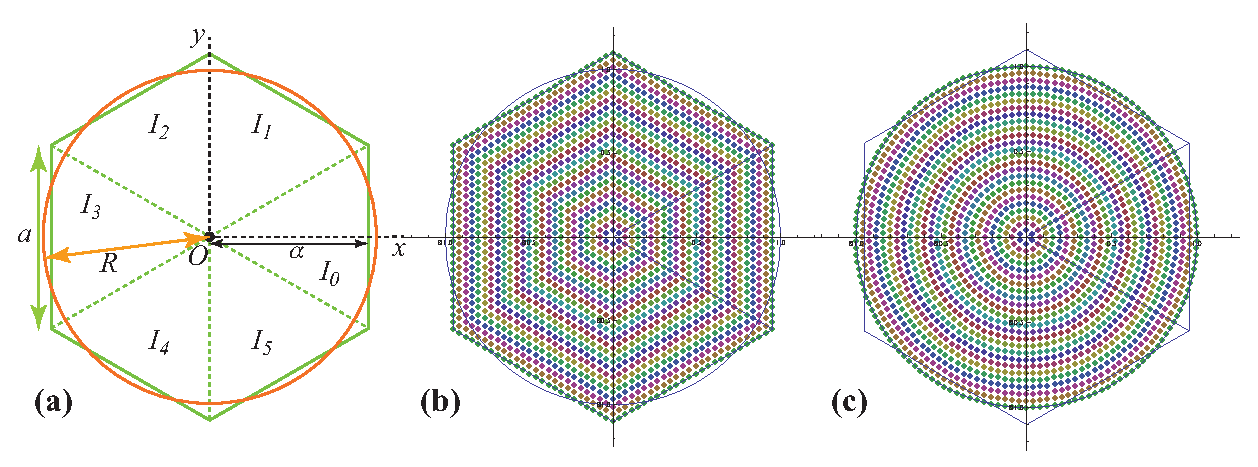
\includegraphics[width=5in]{figs/hextest}
\caption{(a) Subdivision of the hexagon into sextants; the circle has the same area as the hexagon; (b) 
shows a uniform grid in the hexagon, and (c) shows the same grid after equal-area mapping onto the circle.} \label{fig:hextest}
\end{figure}

The point $(x,y)\neq(0,0)$ in the circle is mapped into $(X,Y)_H$ in the hexagon with coordinates given by
\begin{itemize}
\item For $(x,y)\in I_0 \cup I_3$,
\begin{equation}\label{a03}
 (X,Y)_H=3^{\frac 14}{\sqrt{\frac 2\pi}}\, x \left(
\cos\frac{y\pi}{2\sqrt{3}x},\sin\frac{y\pi}{2\sqrt{3}x}\right);
\end{equation}
\item For $(x,y)\in I_1 \cup I_4$,
\begin{equation}\label{a14}
 (X,Y)_H = \frac{3^{\frac 14}}{\sqrt{2\pi}} (x+\sqrt 3y) \left(
\sin\frac{2\pi x}{3(x+\sqrt{3}y)},\ \cos\frac{2\pi
x}{3(x+\sqrt{3}y)}\right);
\end{equation}
\item For $(x,y)\in I_2 \cup I_5$,
\begin{equation}\label{a25}
 (X,Y)_H = \frac{3^{\frac 14}}{\sqrt{2\pi}} (x-\sqrt 3y) \left(
\sin\frac{2\pi x}{3(x-\sqrt{3}y)},-\cos\frac{2\pi
x}{3(x-\sqrt{3}y)}\right).
\end{equation}
\end{itemize}
For the origin we define $\mathcal T_H(0,0)=(0,0)$.  The inverse transformation is given by:
\begin{itemize}
\item For $(X,Y)\in I_0\cup I_3$
\begin{equation}\label{f03}
 (x,y)=3^{-\frac 14}\sqrt {X^2+Y^2}\,\mbox{sign}(X)\left(
\sqrt{\frac \pi 2},\,\sqrt{\frac 6\pi} \arctan \frac YX \right);
\end{equation}
\item For $(X,Y)\in I_1\cup I_4$,
\begin{equation}\label{f14}
 (x,y)=\frac{3^\frac 14\sqrt {X^2+Y^2}}{\sqrt
{2\pi}}\,\mbox{sign}(X)\left(
\sqrt3\Big(\frac \pi 6-\arctan \frac{Y-\sqrt 3 X}{X+\sqrt 3 Y}\,\Big),
\frac \pi 2+\arctan \frac{Y-\sqrt 3 X}{X+\sqrt 3 Y} \right);
\end{equation}
\item For $(X,Y)\in I_2\cup I_5$,
\begin{equation}\label{f25}
 (x,y)=\frac{3^\frac 14\sqrt {X^2+Y^2}}{\sqrt
{2\pi}}\,\mbox{sign}(X)\left(
\sqrt3\Big(\frac \pi 6+\arctan \frac{Y+\sqrt 3 X}{X-\sqrt 3 Y}\,\Big),
-\frac \pi 2+\arctan \frac{Y+\sqrt 3 X}{X-\sqrt 3Y} \right).
\end{equation}
\end{itemize}
The coordinates in the circle can then be transported onto the Northern unit hemisphere by the 
following inverse Lambert projection:
\begin{equation}
 (\widetilde{x},\widetilde{y},\widetilde{z}) =
\left(\frac{x}{2}\sqrt{4-(x^2+y^2)} ,\frac{y}{2}\sqrt{4-(x^2+y^2)}, 1-\frac{1}{2}(x^2+y^2)\right).\label{eq:lama}
\end{equation}
This relation assumes that the radius of the circle is defined as $R=\sqrt{2}$.
The Lambert projection from the hemisphere to the circle is then given by:
\begin{equation}
    (x,y) = \sqrt{\frac{2}{1+\widetilde{z}}} \left(\widetilde{x},\widetilde{y} \right);\label{eq:lamb}
\end{equation}
For all these relations to work together, we must also have $a=2\sqrt \pi 3^{-3/4}$ for the hexagon edge
length, and therefore $\alpha=3^{1/4}\sqrt{\pi}$ (see Fig.~\ref{fig:hextest}).  This completes the discussion 
of the equal area projections used in the EBSD software.

\subsection{Master Pattern Symmetry \label{sec:Laue}}
In the previous version of the EBSD master program, we had implemented the $11$ Laue groups as the possible 
symmetries for the master pattern.  Implicitly, however, this meant that we were applying Friedel's Law, which 
states that all kinematical diffraction patterns are centro-symmetric, hence the use of the Laue groups. For the 
dynamical EBSD pattern simulations, however, it turns out that this is incorrect.  So, in the present version of the 
program, we have corrected this problem, and now the full point group symmetry is properly taken into account;
as a result, the code has become quite a bit more complicated.

There are $32$ crystallographic point group symmetries, and each of them requires a dedicated k-space sampling scheme, using the Lambert projections described above.
For the crystal systems that map onto the square Lambert projection, things are the same as before, except that we now need to use 
two Lambert maps, one for the Northern hemisphere, one for the Southern; in the absence of inversion symmetry, both are needed.
For the trigonal and hexagonal cases the situation has become quite complicated due to the fact that the trigonal groups can be
considered both with a hexagonal and a rombohedral setting.  In addition, for the trigonal/rhombohedral case, the three-fold 
rotation axis does not coincide with the reciprocal $\mathbf{c}^{\ast}$ axis, but instead is aligned with the trigonal $[111]$ direction, 
which causes a bit of a problem.  In addition, for both the tetragonal and hexagonal crystal systems, there is one point group
that has two settings ($\bar{4}2m/\bar{4}m2$ and $\bar{6}m2/\bar{6}2m$), and this must be taken into account when deciding 
what the asymmetric unit is for k-space sampling.

Fig.~\ref{fig:hemispheres} shows the $42$ cases for all point group settings; for each case, two circles are shown, representing the 
stereographic projections of the Northern and Southern hemispheres, labeled $NH$ and $SH$; the green number between the two
circles is the point group number.  The black number on the left indicates the case number, whereas the red number to the right of $SH$
indicates the unique case number; several cases end up having the same sampling scheme.  So, in total, there are 19 unique
sampling schemes; these are implemented in the \textsf{kvectors} module.  To determine the proper sampling scheme, the 
\textsf{EMEBSDmaster} program uses both the space group number and the point group symmetry; this is all done automatically
behind the scenes.  In cases where the SH projection is blank, this means that all points in this projection are generated from the 
corresponding NH section by symmetry operations.

Note that for the cubic symmetry groups, we use lower symmetry cases to make sure that the complete square Lambert array
is properly filled without interpolations.  This means that cubic symmetry takes longer to compute than it should, and we are 
actively researching alternative approaches that would permit the highest possible resolution Lambert projections for the 
shortest possible execution time.

For the (obverse) rhombohedral setting of the trigonal space groups, the implementation of the Lambert projections has 
not yet been worked out; this should not be a problem, since those space groups can always be treated in the hexagonal
setting.  A full symmetry implementation for the obverse rhombohedral case will become available in one of the next releases
of \textsf{EMSoft}.  The main issue preventing a simple implementation is the fact that the center axis of the Lambert projection
is always taken along $\mathbf{c}^{\ast}$, whereas the highest symmetry rotation axis in the rhombohedral case lies along the 
$[111]_r$ direction, which obviously does not coincide with $\mathbf{c}^{\ast}$.  This will require special treatment, most likely 
via the coordinate transformation relating the rhombohedral and hexagonal settings (not difficult, but sufficiently different 
from the treatment of the other point groups that some special code will be required).

\begin{figure}[t]
\centering\leavevmode
\epsfxsize=6.5in\epsffile{figs/hemispheres}
\caption{\label{fig:hemispheres}Asymmetric units for the $32$ point groups, drawn on Northern and Southern stereographic projections.}
\end{figure}

%
%For the rhombohedral setting of the trigonal space groups, a problem arises: the three-fold rotation axis lies along the 
%trigonal $[111]$ direction, not along the $\mathbf{c}^{\ast}$ axis, as is the case for nearly all other symmetry groups. To apply the 
%symmetry operations in the context of the master pattern approach, we must rotate the asymmetric sampling unit to fall 
%around the threefold axis, but this axis does not lie at the center of the master pattern. This is not an easy case to implement.
%On the one hand, the hexagonal Lambert projection requires the three-fold axis to lie at the pattern center. On the other hand,
%for a given set of trigonal lattice parameters, $(a,\alpha)$, in rhombohedral setting, in the standard crystallographic orientation
%the $\mathbf{c}^{\ast}$ axis will lie at the pattern center.  To properly apply the trigonal symmetry, we must determine the 
%transformation that takes a $\mathbf{k}$ vector between the two coordinate systems.  The $\mathbf{a}$ and $\mathbf{b}$ axes
%lie in the plane of the Lambert projection, with an angle $\alpha$ between them.  It is not too difficult to figure out how to
%map the rhombohedral system onto the hexagonal Lambert grid.  First, the $[111]_r$ direction must be rotated into the $x-z$
%plane by a counterclockwise rotation around the $x$ axis by an angle that depends on the rhombohedral $\alpha$ angle; the 
%corresponding rotation matrix is given by:
%\begin{equation}
%	R_x(\alpha) = \left(\begin{array}{ccc}
%	1 & 0 & 0\\
%	0 & x & -\sqrt{1-x^2}\\
%	0 & \sqrt{1-x^2} & x\end{array}\right)\qquad\text{with}\quad x\equiv\frac{1}{2}\sec\frac{\alpha}{2}.
%\end{equation}
%Then the rotated $[111]_r$ must be rotated clockwise around the $y$ axis by the following matrix:
%\begin{equation}
%	R_y(\alpha) = \left(\begin{array}{ccc}
%	y & 0 & -\sqrt{1-y^2}\\
%	0 & 1 & 0\\
%	\sqrt{1-y^2} & 0 & y\end{array}\right)\qquad\text{with}\quad y\equiv\frac{2}{\sqrt{3}}\sin\frac{\alpha}{2}.
%\end{equation}
%The complete transformation matrix (called \textsf{trigmat} in the \textsf{cell} structure), is then given by
%the product:
%\begin{equation}
%	t = R_y(\alpha) R_x(\alpha) d(a,\alpha)
%\end{equation}
%where $d(a,\alpha)$ is the direct structure matrix for the rhombohedral system:
%\begin{equation}
%	d(a,\alpha)\equiv = a\left(\begin{array}{ccc}
%	1 & \cos\alpha & \cos\alpha \\
%	0 & \sin\alpha & -\cos\alpha\tan\frac{\alpha}{2}\\
%	0 & 0 & \tan\frac{\alpha}{2}\sqrt{2\cos\alpha+1}\end{array}\right).
%\end{equation}
%Application of the matrix $t$ to the rhombohedral direction $[111]_r$ produces a vector along the $z$ direction normal to the 
%hexagonal Lambert projection; application to $[100]_r$ produces a vector in the $x-z$ plane.

\subsection{Hexagonal Lambert patterns \label{sec:hexagonal}}
For the hexagonal and trigonal Laue symmetries, the \textsf{EMEBSDmaster} and \textsf{ECPmaster} programs sample the electron beam directions on 
a hexagonal grid, so that the symmetry elements can be implemented properly.  Subsequently, this grid is transformed to a standard
square grid for further processing in the \textsf{EMEBSD}/\textsf{EMECP} programs.  This transformation is achieved by going through the square grid, 
for each point determining the unit vector on the projection hemisphere, and then projecting down into the hexagonal grid using 
bilinear interpolation.  The output of the \textsf{EMEBSDmaster}/\textsf{EMECPmaster} programs is all encoded on the square Lambert grid; the hexagonal
grid is only used inside this program and is not visible to the user.


%e transformation is performed using barycentric coordinates\footnote{See, for
%instance, \textit{http://en.wikipedia.org/wiki/Barycentric\_coordinate\_system} or \textit{http://mathworld.wolfram.com/ BarycentricCoordinates.html} for details.}
%for the interpolation.  Referring to the hexagonal and square grids in Fig.~\ref{fig:bary}, 
%the interpolated intensity $I_p(h)$ in a point that lies a 
%distance $h$ above the base $1$--$2$ of a triangle with top $3$ is given by:
%\[
%	I_p(h) = (I_1+I_2)\lambda+(1-2\lambda) I_3\quad\text{with}\quad \lambda=\frac{1}{2} - \frac{h}{\delta\sqrt{3}},
%\]
%where $\delta$ is the step size along the horizontal direction.  The hexagonal grid points $(i,j)$ then 
%lie on cartesian positions with coordinates $(x,y)=(i_h\delta-j_h\delta/2,j_h\delta\sqrt{3}/2)$.  With the exception of 
%the grid points with $j_h=0$, the value of $h$ is always non-zero.  It is not too difficult to distinguish between
%triangles with apex $3$ pointing upward or downward.
%
%\begin{figure}[h]
%\centering
%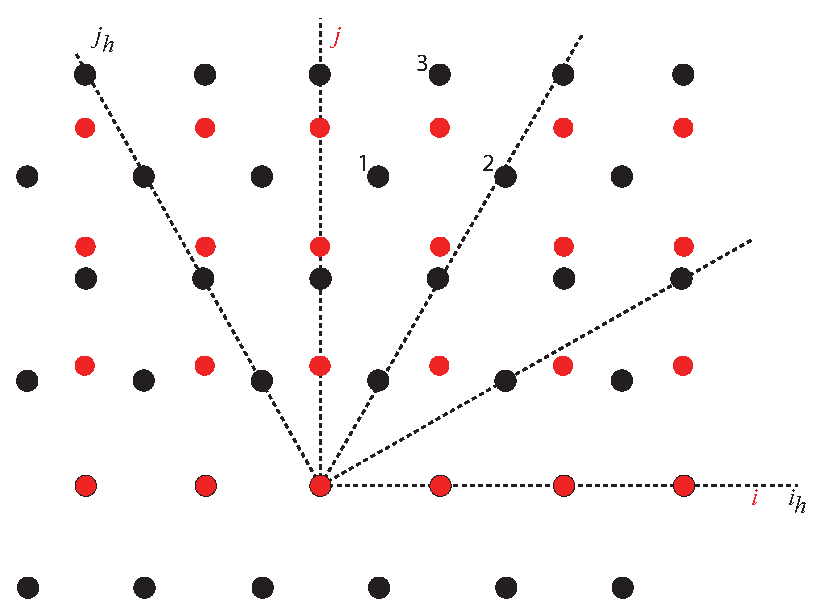
\includegraphics[width=4in]{figs/bary}
%\caption{Correspondence between hexagonal and square sampling grids used for barycentric interpolation.} \label{fig:bary}
%\end{figure}
%
%Summarizing, the master pattern for structures with hexagonal or trigonal symmetry is computed by sampling incident beam directions
%on a hexagonal grid (limited to the corresponding asymmetric unit); these grid points correspond to incident beam directions according 
%to the modified Lambert mapping introduced in section~\ref{sec:Lambert}.  Once all EBSD intensities have been computed, the symmetry
%elements are applied, and the hexagonal grid is interpolated onto a standard square grid using the barycentric approach described above.
%From then on, there is no further need for a distinction between hexagonal/trigonal and other symmetries (i.e., only the master pattern
%computation in \textsf{EMEBSDmaster} needs to distinguish between the different Laue symmetries).
%
%{\color{blue}Note that at the time of writing of this manual, the hexagonal/trigonal case is not yet completely validated; this is ongoing work
%and the source files will be updated if modifications are needed.}

\newpage
\subsection{Monte Carlo Simulations \label{sec:MC}}
The current implementation of the Monte Carlo code makes use of the Continuous Slowing Down Approximation (CSDA),
which assumes that the incident electron loses energy at a constant rate as it travels inside the sample.  This is obviously a
rather coarse approximation, since core losses, outer shell excitations, plasmons, phonons, etc are not taken into account
explicitly, but replaced by a constant energy loss rate.  From a modeling point of view, on the other hand, it is relatively easy
to implement, so we have selected this as a first approximate approach over a more involved Monte Carlo model that has been
under development as well.  

In the Monte Carlo approach, we consider each beam electron separately and follow it on a stochastic trajectory 
through the sample.  The electron travels a random distance scaled by the mean free path length, and then undergoes a 
scattering event which changes the direction cosines of the trajectory; this process is repeated until either the electron has
lost more than a preset amount of energy, or the electron leaves the sample, at which point the direction cosines, energy,
and depth of the last scattering event are noted.  From this information, the program then generates two different data sets:
\begin{itemize}
	\item the spatial distribution of electrons, represented on a modified Lambert projection, for each of a series of 
	energy bins;
	\item and the depth distribution vs.\ energy and orientation.
\end{itemize}
This data is then used by the  EMEBSDmaster simulation program to determine the depth integration limits and the probability 
that an electron with a given energy was backscattered at a given depth (note that the depth is the effective distance traveled 
inside the sample after the last scattering event).  For more details on the Monte Carlo approach we refer the interested reader to
the literature.\footnote{Heinrich, K.H.J., Newbury, D.E. \& Yakowitz, H. (Eds.) (1975).
\textit{Use of Monte Carlo Calculations in Electron Probe Microanalysis and Scanning Electron Microscopy} Gaithersburg, MD: National Bureau of Standards;
Joy, D.C. (1995). \textit{Monte Carlo Modeling for Electron Microscopy and Microanalysis} New York: Oxford University Press.}

In version 3.x, the core of this Monte Carlo simulation is performed on a GPU platform, if one is available, using an OpenCL kernel.  The kernel source code 
must be available in the proper folder, EMSoftpathname/opencl.

Note also that this program can be used to perform simulations both for the EBSD case and for the ECP case; this will be discussed in more 
detail in section~\ref{sec:f90MC}.

\subsection{Master EBSD and ECP Pattern Simulations \label{sec:Master}}
For the master pattern we employ the Bloch wave approach combined with a depth integration.  The probability 
of back-scattered electrons originating from the sample along a specific direction must be integrated over the depth
along that direction, which involves an integral over depth.  In our approach, this integral is replaced by a summation
over the depth bins generated in the \textsf{EMMCOpenCL} program.  

The probability of scattering from each subset $\mathcal{S}$ of atomic sites within the 
unit cell for a given incident beam direction $\mathbf{k}_0$ and an exit energy $E$ can be written as:
\begin{equation}
\mathcal{P}(\mathbf{k}_0, E) = \sum_{\mathbf{g}}\sum_{\mathbf{h}} S_{\mathbf{g}\mathbf{h}}L_{\mathbf{g}\mathbf{h}}(E),
    \label{eq:prob}
\end{equation}
with
\begin{subequations}
\begin{align}
    S_{\mathbf{g}\mathbf{h}} &\equiv \sum_{n}\sum_{i\in\mathcal{S}_n} Z^2_n\,e^{-M^{(n)}_{\mathbf{h}-\mathbf{g}}}\,e^{2\pi\mathrm{i} 
    (\mathbf{h}-\mathbf{g})\cdot\mathbf{r}_{i}};\label{eq:defa}\\
    L_{\mathbf{g}\mathbf{h}}(E) &\equiv \sum_{j}\sum_{k} 
    C^{(j)\ast}_{\mathbf{g}}\alpha^{(j)\ast}\mathcal{I}_{jk}(E)\alpha^{(k)}
    C^{(k)}_{\mathbf{h}}.\label{eq:defb}
\end{align}
\end{subequations}
The first summation in (\ref{eq:defa}) runs over all the positions in the asymmetric unit of the unit cell; the second
sum runs over all equivalent positions in each subset $\mathcal{S}_n$.
The parameters $\alpha^{(j)}$ in (\ref{eq:defb}) are the Bloch wave excitation amplitudes, $C_{\mathbf{g}}^{(j)}$ are the 
Bloch wave coefficients, and the matrix $\mathcal{I}_{jk}$ is defined by the integral
\begin{equation}
	\mathcal{I}_{jk}(E)\equiv \frac{1}{z(E)}\int\limits_{0}^{z(E)} 
    \lambda(E,z) e^{-2\pi(\alpha_{jk}+\mathrm{i}\beta_{jk})z}\,\mathrm{d}z,
\end{equation}
where $z(E)$ and $\lambda(E,z)$ are, respectively, the integration depth and the depth- and 
energy-dependent scattering probability derived from the Monte Carlo program output,
and
\begin{subequations}
\begin{align}
    \alpha_{jk} &= q^{(j)}+q^{(k)};\\
    \beta_{jk} &= \gamma^{(j)}-\gamma^{(k)}.
\end{align}
\end{subequations}
The complex numbers $\lambda^{(j)}\equiv\gamma^{(j)}+\mathrm{i}q^{(j)}$ are the eigenvalues of the dynamical scattering matrix in the 
presence of absorption.  The integration is performed numerically by simply summing the result for a discrete series of depths.
The resulting data is stored as a modified Lambert projection grid (see previous sections).  

The only difference between the EBSD and ECP cases is the fact that for the ECPs there is only one energy to consider,
whereas the EBSD patterns require integration over an energy range; this means that the $z(E)$ and $\lambda(E,z)$
functions are different for EBSD and ECP.  Otherwise, the two simulations approaches are nearly identical.
{\small
In a later release, we will replace the Bloch wave approach by an equivalent scattering matrix approach, so that we can use the GPU platform
to compute the necessary matrix exponentials.  The Bloch wave approach requires an OpenCL version of the Lapack routines
which we have not been able to get to work thus far.  The derivation proceeds as follows.

Application of the scattering matrix approach to the EBSD modality requires a different ``Ansatz'' for the wave 
function $\Psi(\mathbf{r})$; we write:
\begin{equation}
	\Psi(\mathbf{r}) = \sum_{\mathbf{g}} \psi_{\mathbf{g}}(\mathbf{r}) 
	\mathrm{e}^{2\pi\mathrm{i}(\mathbf{k}_0+\mathbf{g})\cdot\mathbf{r}};\label{eq:planewaves}
\end{equation}
this expression implicitly assumes that the scattered electron can only travel along the directions predicted by the 
Bragg equation, $\mathbf{k}'=\mathbf{k}_0+\mathbf{g}$.  After substitution in the perfect crystal Schr\"odinger equation,
application of the high energy approximation, and the substitution:
\begin{equation}
	\psi_\mathbf{g}(\mathbf{r}) = S_{\mathbf{g}}(\mathbf{r}) \mathrm{e}^{\mathrm{i}\theta_{\mathbf{g}}},\label{eq:psig}
\end{equation}
where $\theta_{\mathbf{g}}$ is the phase of the Fourier coefficient $U_{\mathbf{g}}$, we obtain the following system of 
coupled first order differential equations:
\begin{equation}
    \frac{\mathrm{d} S_{\mathbf{g}}(z)}{\mathrm{d}z} =
    2\pi\mathrm{i}s_{\mathbf{g}}S_{\mathbf{g}}(z) + \mathrm{i}\pi {\sum_{\mathbf{g}'}}
    \frac{1}
    {q_{\mathbf{g}-\mathbf{g}'}}S_{\mathbf{g}'}(z),\label{eq:defectequation}
\end{equation}
where
\begin{equation}
	\frac{1}{q_{\mathbf{g}}} \equiv \frac{1}{\xi_{\mathbf{g}}} + \mathrm{i}
	\frac{\mathrm{e}^{\mathrm{i} (\theta^{\prime}_{\mathbf{g}}-\theta_{\mathbf{g}})}}{\xi^{\prime}_{\mathbf{g}}};
	\label{eq:defineq}
\end{equation}
the extinction distance $\xi_{\mathbf{g}}$ and anomalous absorption length $\xi'_{\mathbf{g}}$ are defined as:
\begin{equation}
	\frac{1}{\xi_{\mathbf{g}}}\equiv \frac{\vert U_{\mathbf{g}}\vert}{\vert\mathbf{k}_0+\mathbf{g}\vert\cos\alpha};\qquad
	\frac{1}{\xi'_{\mathbf{g}}}\equiv \frac{\vert U'_{\mathbf{g}}\vert}{\vert\mathbf{k}_0+\mathbf{g}\vert\cos\alpha};
\end{equation}
$U_{\mathbf{g}} = (2me/h^2) V_{\mathbf{g}} $, $\alpha$ is the angle between the beam direction and $\mathbf{k}_0+\mathbf{g}$, and $\mathbf{k}_0$ is 
the incident wave vector corrected for refraction.  The absorption potential Fourier coefficients are represented by $U'_{\mathbf{g}} = (2me/h^2) V'_{\mathbf{g}}$.

This set of equations can be represented in matrix form as:
\begin{equation}
	\frac{\mathrm{d}\mathbf{S}(z)}{\mathrm{d}z} = \mathrm{i}\mathcal{A}(\mathbf{r})\mathbf{S}(z),\label{eq:matrix}
\end{equation}
where the structure matrix $\mathcal{A}$ contains the excitation errors and the normal absorption coefficient $1/q_{\mathbf{0}}$ 
along its diagonal, and the interaction parameters $1/q_{\mathbf{g}}$ on the off-diagonal positions:
\begin{align*}
    \mathcal{A}_{\mathbf{g},\mathbf{g}} & = 2\pi s_{\mathbf{g}} + \frac{\pi}{q_{\mathbf{0}}};\\
    \mathcal{A}_{\mathbf{g},\mathbf{g}'} & = \frac{\pi}{q_{\mathbf{g}-\mathbf{g}'}}.
\end{align*}
The formal solution for a crystal of thickness $\epsilon$ is then given by:
\begin{equation}
	\mathbf{S}(\epsilon) = e^{\mathrm{i}\mathcal{A}\epsilon}\mathbf{S}(0) = \mathcal{S}(\epsilon)\mathbf{S}(0);
\end{equation}
the matrix exponential $\mathcal{S}(z)$ is commonly known as the \textit{scattering matrix}, and can be computed numerically
by means of the Pad\'e approximation \cite{moler2003a}.

Substitution of eq.~(\ref{eq:planewaves}) into the BSE yield equation results in the following expression 
for the BSE yield:
\begin{equation}
	\mathcal{P}(\mathbf{k}_0) = \frac{1}{z_0}\sum_{n}\sum_{i\in\mathcal{S}_n}\sum_{\mathbf{g}}\sum_{\mathbf{h}} \int\limits_{0}^{z_{0}} \mathrm{d}z\,
	 Z^2_n\,\mathrm{e}^{-M^{(n)}_{\mathbf{h}-\mathbf{g}}}\,\mathrm{e}^{2\pi\mathrm{i} (\mathbf{h}-\mathbf{g})\cdot\mathbf{r}_{i}} 
%	\mathrm{e}^{\mathrm{i}(\theta_{\mathbf{h}}-\theta_{\mathbf{g}})} 
	S^{\ast}_{\mathbf{g}}(z) S_{\mathbf{h}}(z).
    \label{eq:prob2}
\end{equation}
This expression can be simplified as for the Boch wave case to read:
\begin{equation}
	\mathcal{P}(\mathbf{k}_0) = \sum_{\mathbf{g}}\sum_{\mathbf{h}} S_{\mathbf{g}\mathbf{h}} L^{S}_{\mathbf{g}\mathbf{h}},
    \label{eq:prob2}
\end{equation}
where the matrices are defined as
\begin{subequations}
\begin{align}
    S_{\mathbf{g}\mathbf{h}} &\equiv \sum_{n}\sum_{i\in\mathcal{S}_n} Z^2_n\,\mathrm{e}^{-M^{(n)}_{\mathbf{h}-\mathbf{g}}}\,\mathrm{e}^{2\pi\mathrm{i} 
    (\mathbf{h}-\mathbf{g})\cdot\mathbf{r}_{i}};\label{eq:defnewa}\\
    L^{S}_{\mathbf{g}\mathbf{h}} &\equiv \frac{1}
    {z_{0}}\int\limits_{0}^{z_{0}} \mathrm{d}z\,  S^{\ast}_{\mathbf{g}}(z) S_{\mathbf{h}}(z).
    \label{eq:defnewb}
\end{align}
\end{subequations}
The superscript $S$ in $L^{S}_{\mathbf{g}\mathbf{h}}$ refers to the scattering matrix approach.  Note that the matrix 
$S_{\mathbf{g}\mathbf{h}}$ is identical to that for the Bloch wave approach in the previous section (eq.~(\ref{eq:defa})).  
As in the Bloch wave case, we must replace the integral above by an energy-dependent depth-weighted integration, as follows:
\begin{equation}
	L^{S}_{\mathbf{g}\mathbf{h}}(E) \equiv  \frac{1}{z(E)}\int\limits_{0}^{z(E)} \mathrm{d}z\,  
    \lambda(E,z) S^{\ast}_{\mathbf{g}}(z) S_{\mathbf{h}}(z).
\end{equation}
The entire computation of the matrix $L$ can then be performed on the GPU, potentially resulting in a tremendous acceleration compared to the 
OpenMP CPU version.  Each OpenCL work-item performs an entire matrix computation, with the limitation that all 
matrices must have the same size (same number of beams); this requires a rather comprehensive rewrite of the fortran-90 
code in the main \textsf{EMEBSDmaster} program, which is currently underway.
}

\begin{figure}[t]
\centering
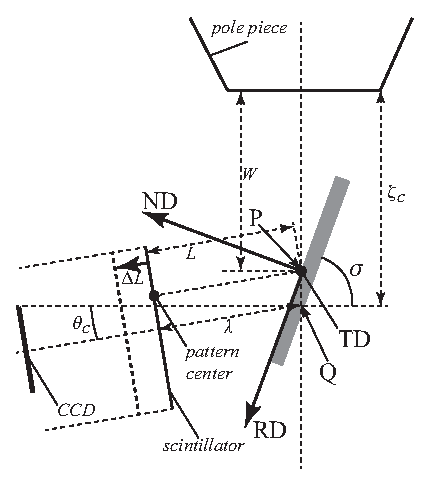
\includegraphics[width=3in]{figs/geometry}
\caption{Typical geometry of sample and scintillator for an EBSD experiment.} \label{fig:geometry}
\end{figure}



\subsection{Final EBSD Pattern Simulations \label{sec:EBSP}}
Consider the geometry in Fig.~\ref{fig:geometry}, which shows the sample-scintillator configuration 
for a typical EBSD experiment.  The diffraction geometry is fully determined if we can express the direction cosines of the line connecting
an arbitrary point on the scintillator screen to the interaction point $P$ on the sample surface, expressed with 
respect to the $(RD,TD,ND)$  triad.  We measure the scintillator coordinates with the $x_s$ axis in the direction 
opposite to TD, and the $y_s$ axis pointing up towards the objective lens.   The $z_s$ axis is then 
normal to the screen and forms a second right-handed unit triad.  These coordinates are measured with 
respect to the center of the screen and can be positive or negative (except for $z_s$ which is always positive).
In the scintillator reference frame, a single point on the screen has coordinates $(x_s,y_s,0)$ and the 
point $Q$ has coordinates $(0,0,\lambda)$.  The interaction point $P$ has coordinates $(x_{pc},y_{pc},L)$.
For simplicity, we will measure all coordinates in units of micrometers ($\mu$m).

The arbitrary point $(x_s,y_s,0)$ on the scintillator screen corresponds to a set of three direction cosines 
with respect to the sample reference frame.   The angle between ND and the scintillator normal is $\alpha=\frac{\pi}{2}-\sigma+\theta_c$.
If the pattern center were located on the ND axis, by rotating the detector assembly by a clockwise angle $\alpha$ around
the TD direction, then its $(RD,TD,ND)$ coordinates (keeping track of the definition of this reference frame) 
would be $(y_{pc}-y_s,x_{pc}-x_s,L)$.  After counterclockwise rotation to the actual camera orientation we 
find for the screen coordinates in the sample reference frame:
\[
	\mathbf{r}_g = \left[ (y_{pc}-y_s)\cos\alpha+L\sin\alpha, x_{pc}-x_s, -(y_{pc}-y_ss)\sin\alpha+L\cos\alpha\right].
\]
The length of this vector is simply:
\[
	\vert \mathbf{r}_g\vert \equiv \rho_s = \sqrt{L^2+(y_{pc}-y_s)^2 + (x_{pc}-x_s)^2}
\]
so that the direction cosines of a screen pixel $(x_s,y_s,0)$ in the (RD,TD,ND) reference frame are given by:
\begin{equation}
	\hat{\mathbf{r}}_g(x_s,y_s) = \frac{\mathbf{r}_g}{\rho_s}.\label{eq:dc}
\end{equation}
For a given crystallographic grain orientation, it is straightforward to convert these
direction cosines to an electron channeling direction (all rotations are implemented by means of quaternion arithmetic in our
implementation).  This transformed direction is then further converted
to coordinates $(X,Y)$ on the square grid of the master EBSD pattern, which is 
used as a look-up table (with appropriate  bi-linear interpolation) for the EBSD intensity at the scintillator
position $(x_s,y_s,0)$.   Repeating this for all scintillator pixels then provides the complete EBSD signal for a given grain orientation.

We represent the energy-dependent master EBSD pattern by the symbol $\mathcal{M}(\kappa,X,Y)$,  where the first component labels the energy bins, 
and $(X,Y)$ indicates the position on the square sampling grid.   The energy histogram from the Monte Carlo simulation is represented by the symbol
$\mathcal{E}(\kappa,i,j)$, where $(i,j)$ references the scintillator pixel $(x_s,y_s)=(i,j)\delta$.  The number of BSE electrons incident on that pixel can then be written as
a weighted sum over all $n_E$ energy bins:
\begin{equation}
	I_{\text{BSE}}(i,j) = \eta\sum_{\kappa=1}^{n_E} s(\kappa)\mathcal{E}(\kappa,i,j) \mathcal{M}\left(\kappa,X(x_s,y_s,\tilde{q}),Y(x_s,y_s,\tilde{q})\right),\label{eq:intensity}
\end{equation}
where $\tilde{q}$ is a unit quaternion that represents the grain orientation (derived from a triplet of Euler angles), and the coordinates 
$(X,Y)$ are computed from $(x_s,y_s)$ and $\tilde{q}$ by the sequential application of equation~(\ref{eq:dc}), the quaternion rotation of the resulting
direction cosines, and the inverse Lambert projection equations.  The prefactor $\eta$ in (\ref{eq:intensity}) is defined as:
\begin{equation}
	\eta = \frac{n_A I_0 \Delta t}{N_{MC}}
\end{equation}
where $I_0$ is the incident probe current in Amperes, $\Delta t$ the dwell time in seconds, $N_{MC}$ is the total number of incident electrons
used for the Monte Carlo simulation, and $n_A=6.241\times 10^{18}$ electrons per Coulomb.  The resulting units for $I_{\text{BSE}}$ are then number of  
electrons incident on the scintillator.  The factor $s(\kappa)$ represents the energy conversion efficiency of the scintillator and is currently set equal to unity
for all energies.

This is not the final EBSD pattern as acquired by the CCD camera.  One must still take into account the point spread function of the 
optics that projects the photons onto the CCD chip, Poisson noise, as well as any binning and contrast/brightness scaling that can 
be applied to the pattern. These final steps are currently not available, %only available in a preliminary form via the IDL visualization interface.
but the simulated patterns already have a satisfactory agreement with experimental observations.




\subsection{Final ECP Pattern Simulations \label{sec:ECP}}
The geometry for the ECP case is quit different from the EBSD case.  First of all, the sample is typically nearly horizontal for ECP,
and, secondly, the detector is an integrating detector, not a position sensitive detector.  Therefore, the ECP is obtained by scanning
the incident beam inside a conical volume with apex as the rocking point on the sample surface, and then measuring the integrated 
detector signal as a function of the incidence direction.  Simulation of this process requires knowledge of the detector acceptance 
angles, which involves the working distance, $W$, and the detector inner and outer radii, $R_i$ and $R_o$.  Furthermore, the sample may be inclined
slightly with respect to the horizontal plane (in particular for ECCI observations), so this must be taken into account in the detector model.
Finally, the incident beam cone opening angle, $\theta_c$, must be specified.  %The basic geometry is depicted in Fig.~\ref{fig:ECPgeometry}.

\subsection{Kossel Pattern Simulations\label{sec:Kossel}}
Kossel patterns represent the probability that an incident beam electron survives as part of the (coherent) beam up to a certain depth in
the sample.  They are computed using the same Bloch wave code that is used for the EBSD master pattern simulation.  The intensity level in 
a Kossel pattern is determined from the Bloch wave eigenvalues and excitation amplitudes by the following expression:
\begin{equation}
	P(z,\mathbf{k}_0) = \sum_j \vert \alpha^{(j)}\vert^2 e^{-4\pi q^{(j)}z}.\label{eq:EKP}
\end{equation}
This computation is then repeated for each of the incident beam directions, and the results are collected and displayed as an 
electron Kossel pattern.  The \textsf{EMKosselMaster} program can be used to compute the master pattern in the same way as for
the \textsf{EMEBSDmaster} and \textsf{EMECPmaster} programs.  The IDL \textsf{SEMDisplay} routine discussed in a later section
has resources for the display of the master pattern as well as the computation of specific Kossel patterns for arbitrary 
crystal orientation.



\section{The \protect\textsf{EMMCOpenCL.f90} program\label{sec:f90MC}}
The Monte Carlo program must be executed first, and takes the following name list as input:
\fvset{frame=lines,formatcom=\color{blue},fontsize=\footnotesize}
\VerbatimInput{../templatefolder/EMMCOpenCL.template}
The program uses OpenCL coding to carry out the simulations on a GPU card if one is available.  The input parameters
include the crystal file name (to compute the theoretical density and average atomic number), the sample
tilt angle with respect to the horizontal direction, a potential tilt around the \textsf{RD} axis, the number of pixels
along the modified Lambert projection edge (should be ``a multiple of $10$ plus one''), the number of incident electrons per computational thread, 
the incident beam energy, the minimum energy to be considered, and the energy interval,
as well as the maximum penetration depth and depth step size to be considered.  The data is then stored in an 
HDF5 file.  It should be noted that the execution time of the 
following program, \textsf{EMEBSDmaster}, is directly determined by how many depth steps and energy bins are selected in the
Monte Carlo computation; the more depth steps/energy bins, the longer the dynamical simulation will take.

It should be noted that this program can provide statistics that are used by two other programs: \textsf{EMEBSDmaster.f90} and
\textsf{EMECPmaster.f90}.  To generate output for the former, the variable \textsf{mode} should be set to \textsf{'full'}, 
and the sample tilt angle from horizontal (\textsf{sig}) should be specified.  For the latter program, the \textsf{mode} should
be set to \textsf{'bse1'}, and the user should provide the parameters \textsf{sigstart}, \textsf{sigend}, and \textsf{sigstep}.  In the 
bse1 mode, the program expects the sample to be oriented normal to the electron beam (\textsf{sigstart=0.0}) initially, and 
then the computation is repeated for increasingly larger sample tilt angles (equivalent to beam tilts).  For each tilt value, the 
OpenCL computation is relatively fast since only BSE1 electrons are considered; the total computation time depends on the 
number of sample tilt values that need to be considered.  For the EBSD case, with \textsf{mode='full'}, the computation 
considers all electrons, both BSE1 and BSE2, since both types contribute to the EBSD pattern; in the ECP case, only the 
BSE1 electrons carry diffraction information, since the BSE2 electrons are fully incoherent with respect to the incident beam,
and the integrating annular detector averages any channeling effects of the electrons on their way out of the sample.

The HDF5 output file contains a number of program parameters
that need to be passed on to the next program, as well as two large arrays that contain the electron distribution in the hemisphere on
the vacuum side of the sample surface, formatted as a modified Lambert projection.  Each energy bin has an individual Lambert 
projection.  The second large output array represents the distribution of electron exit depth as a function of energy bin and
orientation, but sampled on a smaller Lambert projection (with one-tenth the number of points along each axis).  This second output
array is used in the \textsf{EMEBSDmaster} program, whereas the first one is primarily used by the \textsf{EMEBSD} program.
%and the IDL display program.

The default number of electrons to be considered is set to $2\times 10^9$; the actual number may be slightly different, due 
to the way the GPU distributes the work to multiple work-items.  In our test runs on the latest generation Mac Pro platform, 
a typical Monte Carlo run takes about $25$ minutes.

Note that all filenames (except for the crystal structure file name) are relative to the \textsf{EMdatapathname} path.  So, if your 
\textsf{EMdatapathname} equals \textsf{/Users/me/EMdata} and you wish the Monte Carlo output file to have the absolute path
\textsf{/Users/me/EMdata/test/MCoutput.h5}, then only the portion \textsf{test/MCoutput.h5} should be entered as the file name
in the name list file.  Relative pathnames are used so that data files can be transferred between computers with different directory
structures.

\section{The \protect\textsf{EMEBSDmaster.f90} and \protect\textsf{EMECPmaster.f90} programs\label{sec:f90EBSDmaster}}
The second program performs the computation of the EBSD master pattern (:or the ECP master pattern) on a
square modified Lambert projection. The input name list file fro the \textsf{EMEBSDmaster} program is formatted as follows:
\fvset{frame=lines,formatcom=\color{blue},fontsize=\footnotesize}
\VerbatimInput{../templatefolder/EMEBSDmaster.template}
For the \textsf{EMECPmaster} program, the input file is nearly identical:
\fvset{frame=lines,formatcom=\color{blue},fontsize=\footnotesize}
\VerbatimInput{../templatefolder/EMECPmaster.template}
The only difference is \textsf{restart} parameter described below.
These short input files only requires the definition of the smallest $d$-spacing to be taken into account 
in the dynamical simulation, the number of pixels along the output Lambert projection, the name of the 
output file from the \textsf{EMMCOpenCL} program, and the name of an HDF5 output file.  The data file from
the Monte Carlo program already contains a lot of other information, so there is no need to duplicate 
any of it in this input file.  This does imply that the Monte Carlo program must be completed before the 
master pattern can be computed.

The \textsf{EMEBSDmaster} program can take a very long time to run, despite the fact that the current version is a multi-threaded OpenMP code.
For each energy bin, a complete EBSD master pattern is computed, using the appropriate asymmetric unit according to
the crystal symmetry.  The output HDF5 file contains a stack of modified Lambert projections, one for each energy bin, along with 
some other parameters.  The size of the Lambert projections does not need to be the same as the size of the Monte Carlo
Lambert projections.  %The projections can be visualized using the IDL program.  
Note that for complex crystal structures,
with multiple atom sites in the asymmetric unit, the program will store the master patterns separately for each entry in the asymmetric unit.
This means that one can, in principle, study the effect of elemental substitutions on EBSD patterns.  The \textsf{EMEBSDmaster}
program can be interrupted at any time, since the master patterns will be written to the HDF5 output file for each energy bin.
The \textsf{restart} parameter (set to \textsf{.FALSE.} by default) must then be set to \textsf{.TRUE.} and the computation will
resume with the pattern for the next energy bin.  It is therefore possible to carry out a few energy bins on one computer, and then
continue the computation on another one (hopefully faster).

The parameter \textsf{dmin} determines a truncation value in direct space, which is effectively a truncation in Fourier space; decreasing
this value below the default will dramatically increase the execution time.  For complex crystal structures, the simulation time will also
increase, since the larger unit cell will automatically generate more reciprocal lattice points inside the truncation sphere.


The \textsf{-t} option to the \textsf{EMEBSDmaster} and \textsf{EMECPmaster} programs will also create a file named \textsf{BetheParameters.template} in
your folder.  Rename this file to \textsf{BetheParameters.nml} and set the following parameters, which have been found to be 
reasonable values for a number of crystal structures and accelerating voltages:
\fvset{frame=lines,formatcom=\color{blue},fontsize=\footnotesize}
\VerbatimInput{../templatefolder/BetheParameters.template}
increasing $c_1$ and $c_2$ will increase the computation time, but will also increase the accuracy of the result. For TEM simulations,
to be released at a later point in time, the values of $c_1$ and $c_2$ will likely need to be increased.


\section{The \protect\textsf{EMEBSD.f90} program\label{sec:f90EBSD}}
The final program takes as input a series of detector characteristics as well as orientations, and uses the output from both \textsf{EMMCOpenCL} and
\textsf{EMEBSDmaster} to compute one or more actual EBSD patterns.  
The easiest way to execute this program is via the IDL interface, but command line execution is also possible.  
The input name list file contains the following entries:
\fvset{frame=lines,formatcom=\color{blue},fontsize=\footnotesize}
\VerbatimInput{../templatefolder/EMEBSD.template}

The program reads the name list file, then Monte Carlo output and master patterns;  then the detector geometry is used to
compute the energy distribution with respect to the scintillator.  This is then used along with the master pattern and the 
orientation information to compute the final EBSD patterns.  For a detailed description of all detector parameters we 
refer the interested reader to both the IDL description in section~\ref{sec:idl} and our paper on the EBSD forward model.\footnote{P.G. Callahan and M. De Graef, 
``Dynamical EBSD Patterns Part I: Pattern Simulations,'' Microscopy and Microanalysis, vol. 19, pp. 1255-1265 (2013)}
The output file contains all EBSPs in full resolution,
and can be read with the IDL visualization program; at that point, the camera point spread function can be included, as well
as binning and brightness/contrast scaling. See section~\ref{sec:idl} for details.

Note that this program can also be used to create so-called EBSD dictionaries.  This is a much more advanced functionality 
that we will not fully detail in the present manual, since it is still under development.  We anticipate that dictionary-type 
computations will become available in the next release (3.1).

The \textsf{outputformat} variable should be kept at the value \textsf{'bin'} for manual program runs; it will take on 
the value \textsf{'gui'} for runs that are controlled by the IDL routine described in section~\ref{sec:idl}.  We recommend
that the \textsf{energyaverage} and \textsf{spatialaverage} variables are kept at their default values; they will be removed 
from the input options in a later release.

\section{The \protect\textsf{EMECP.f90} program\label{sec:f90ECP}}
The \textsf{EMECP} program uses the following template file:
\fvset{frame=lines,formatcom=\color{blue},fontsize=\footnotesize}
\VerbatimInput{../templatefolder/EMECP.template}
Note that the bottom set of parameters can be completely ignored in this version of the software.  Most of the parameters 
are similar to the ones in the EBSD case, except for several of the detector parameters.  The \textsf{EMECP} program
can be called from the command line with an input file of this form, or it can be called directly from within the IDL GUI
described in section~\ref{sec:idl}.  

\section{The \protect\textsf{EMKosselMaster} program\label{sec:f90Kossel}}
The \textsf{EMKosselMaster} program does not require any Monte Carlo simulations, and is controlled via
the following namelist template file:
\fvset{frame=lines,formatcom=\color{blue},fontsize=\footnotesize}
\VerbatimInput{../templatefolder/EMKosselMaster.template}
Most of the parameters should be clear from the previous sections.  The \textsf{Kosselmode} parameter is set to 
\textsf{'normal'} to compute a thickness-dependent Kossel master pattern; when the option is set to \textsf{'thicks'},
the output is a single master pattern (as always in HDF5 format) that represents the depth at which the probability 
defined in section~\ref{sec:Kossel} is equal to the value set by the \textsf{tfraction} parameter.  The Kossel master
pattern can be visualized by the \textsf{SEMDisplay} program; for now, only the patterns from the \textsf{'normal'}
mode can be visualized using this interface.




\section{Calling \textsf{EMEBSD} and \textsf{EMECP} from another program\label{sec:external}}
With the creation of release 3.0, we have changed the library format from static to shared, so that the main package
library now has the name (on Mac OS X) \textsf{EMSoftLib.dylib}.  As a direct consequence of this change, several of 
the subroutines can now be called from other languages.  In the present release (3.0), we make two of those routines
available to the user: \textsf{SingleEBSDpatternWrapper} and \textsf{SingleECPatternWrapper}. Each of these routines
takes two arguments, \textsf{argc} and \textsf{argv}, where \textsf{argc} is the number of arguments ($6$ in each case)
and \textsf{argv} contains a series of pointers to each of the arrays that need to be passed on to the wrapper routines.

Note that this has only been tested on Mac OS X with the gfortran 5.2.0 compiler and IDL's \textsf{call\_external} functionality.
There are no guarantees that this will work with other configurations, but we would appreciate any feedback, error messages, and
so forth so that we can work towards making these routines more generally available for direct linking between programs.

The wrapper routines have the following function definitions:
\begin{verbatim}
function SingleEBSDPatternWrapper(argc, argv) bind(c, name='SingleEBSDPatternWrapper') 

use,INTRINSIC :: ISO_C_BINDING

IMPLICIT NONE

INTEGER(c_size_t), VALUE, INTENT(IN)            :: argc 
type(c_ptr), dimension(argc), INTENT(INOUT)     :: argv
REAL(c_float)                                   :: SingleEBSDPatternWrapper
\end{verbatim}
and
\begin{verbatim}
function SingleECPatternWrapper(argc, argv) bind(c, name='SingleECPatternWrapper') 
	
use,INTRINSIC :: ISO_C_BINDING

IMPLICIT NONE

INTEGER(c_size_t), VALUE, INTENT(IN)            :: argc 
type(c_ptr), dimension(argc), INTENT(INOUT)     :: argv
REAL(c_float)                                  		:: SingleECPatternWrapper
\end{verbatim}
and use the fortran 2003 \textsf{ISO\_C\_BINDING} module; each function returns a single 4-byte real which is equal to $1.0$ when the 
function properly returns.  The computed 
EBSD or ECP pattern is returned via a pointer to the corresponding array.  Each function takes a list of $6$ \textsf{c\_ptr}s
in the \textsf{argv} input array.  The order of the pointers is the same for each function but the structure of the arrays is different.  Note that
the \textsf{accum\_e}, \textsf{mLPNH} and \textsf{mLPSH} arrays must be read from the Monte Carlo and master pattern HDF5 files and
passed on to the wrapper routine. 

\subsection{EBSD pattern calculation}
The pointers that are passed on to the EBSD pattern calculation wrapper routine must point to the following arrays:
\begin{enumerate}
	\item \textsf{ipar}: an array of $6$ integers of fortran type \textsf{c\_size\_t} ($8$-byte integers) that represent the array dimensions
	of the other input arrays.  The components of \textsf{ipar} are:
		\begin{enumerate}
			\item[\textsf{ipar}(1)] if $0$, then the complete detector geometry is computed; if $1$, then the stored detector geometry is used.  This is useful (i.e., speeds things up a little)
			when the geometry does not change between consecutive pattern simulations.
			\item[\textsf{ipar}(2)] number of scintillator pixels $s_x$ along horizontal direction
			\item[\textsf{ipar}(3)] number of scintillator pixels $s_y$ along vertical direction
			\item[\textsf{ipar}(4)] number of energy bins $n_E$ in Monte Carlo \textsf{accum\_e} array
			\item[\textsf{ipar}(5)] number $n_{mc}$ of x or y pixels in Monte Carlo \textsf{accum\_e} array (total $2n_{mc}+1$)
			\item[\textsf{ipar}(6)] number $n_{mp}$ of pixels in modified Lambert projected EBSD master pattern (total $2n_{mp}+1$)
		\end{enumerate}
	\item \textsf{fpar}: an array of $13$ floating point numbers of the type \textsf{c\_float} (4-byte reals) that represent several detector geometry parameters. The 
	components of \textsf{fpar} are:
	\begin{enumerate}
		\item[\textsf{fpar}(1)] pattern center x-coordinate [in units of scintillator pixels]
		\item[\textsf{fpar}(2)] pattern center y-coordinate
		\item[\textsf{fpar}(3)] scintillator pixel size [microns]
		\item[\textsf{fpar}(4)] sample tilt angle from Monte Carlo simulation [degrees]
		\item[\textsf{fpar}(5)] sample rotation angle around the RD direction [degrees]
		\item[\textsf{fpar}(6)] detector inclination angle with respect to horizontal [degrees; positive below horizontal]
		\item[\textsf{fpar}(7)] distance between illuminated point and pattern center [micron]
		\item[\textsf{fpar}(8)] beam current [nA]
		\item[\textsf{fpar}(9)] dwell time [micro s]
		\item[\textsf{fpar}(10-13)] quaternion components representing crystal orientation [scalar part first, then vector part]
	\end{enumerate}
	\item \textsf{EBSDpattern}: a floating point array of type \textsf{c\_float} with dimensions $s_x\times s_y$; memory must be allocated by the calling program.
	\item \textsf{accum\_e}: a floating point array with the output from the Monte Carlo program; array dimensions $n_E\times n_{mc}\times n_{mc}$.
	\item \textsf{mLPNH}: a floating point array with the Northern hemisphere portion of the EBSD master pattern; array dimensions $n_{mp}\times n_{mp}\times n_E$.
	\item \textsf{mLPSH}: a floating point array with the Southern hemisphere portion of the EBSD master pattern; array dimensions $n_{mp}\times n_{mp}\times n_E$.
\end{enumerate}
Note that all six arrays must be properly defined by the calling program, and the pointer must be passed in the stated order in the \textsf{argv} array.

\newpage
\subsection{ECP pattern calculation}
The pointers that are passed on to the ECP pattern calculation wrapper routine must point to the following arrays:
\begin{enumerate}
	\item \textsf{ipar}: an array of $7$ integers of fortran type \textsf{c\_size\_t} ($8$-byte integers) that represent the array dimensions
	of the other input arrays.  The components of \textsf{ipar} are:
		\begin{enumerate}
			\item[\textsf{ipar}(1)] if $0$, then the complete detector geometry is computed; if $1$, then the stored detector geometry is used.  This is useful (i.e., speeds things up a little)
			when the geometry does not change between consecutive pattern simulations.
			\item[\textsf{ipar}(2)] number of ECP pattern pixels $s_x$ along horizontal direction
			\item[\textsf{ipar}(3)] number of ECP pattern pixels $s_y$ along vertical direction
			\item[\textsf{ipar}(4)] number of sample tilt angles $n_s$ in Monte Carlo \textsf{accum\_e} array
			\item[\textsf{ipar}(5)] number $n_{mc}$ of x or y pixels in Monte Carlo \textsf{accum\_e} array (total $2n_{mc}+1$)
			\item[\textsf{ipar}(6)] number $n_{set}$ of independent atom positions for which a master pattern is available
			\item[\textsf{ipar}(7)] number $n_{mp}$ of pixels in modified Lambert projected EBSD master pattern (total $2n_{mp}+1$)
		\end{enumerate}
	\item \textsf{fpar}: an array of $12$ floating point numbers of the type \textsf{c\_float} (4-byte reals) that represent several detector geometry parameters. The 
	components of \textsf{fpar} are:
	\begin{enumerate}
		\item[\textsf{fpar}(1)] illumination cone semi-opening angle [degrees]
		\item[\textsf{fpar}(2)] sample tilt angle around RD axis [degrees]
		\item[\textsf{fpar}(3)] working distance [mm]
		\item[\textsf{fpar}(4)] inner radius of BSE detector [mm]
		\item[\textsf{fpar}(5)] outer radius of BSE detector [mm]
		\item[\textsf{fpar}(6)] start angle from Monte Carlo input file [degrees]
		\item[\textsf{fpar}(7)] end angle from Monte Carlo input file [degrees]
		\item[\textsf{fpar}(8)] angle step size from Monte Carlo input file [degrees]
		\item[\textsf{fpar}(9-12)] quaternion components representing crystal orientation [scalar part first, then vector part]
	\end{enumerate}
	\item \textsf{ECpattern}: a floating point array of type \textsf{c\_float} with dimensions $s_x\times s_y$; memory must be allocated by the calling program.
	\item \textsf{accum\_e}: a floating point array with the output from the Monte Carlo program; array dimensions $n_{s}\times n_{mc}\times n_{mc}$.
	\item \textsf{mLPNH}: a floating point array with the Northern hemisphere portion of the ECP master pattern; array dimensions $n_{mp}\times n_{mp}\times n_{set}$.
	\item \textsf{mLPSH}: a floating point array with the Southern hemisphere portion of the ECP master pattern; array dimensions $n_{mp}\times n_{mp}\times n_{set}$.
\end{enumerate}
Note that all six arrays must be properly defined by the calling program, and the pointer must be passed in the stated order in the \textsf{argv} array.



\newpage
\section{The IDL \protect\textsf{SEMDisplay.pro} program\label{sec:idl}}
The \textsf{SEMDisplay.pro} program\footnote{The \ctp\ executable package comes with several virtual machine apps (VMAPPs), 
i.e., pre-compiled IDL routines that can be executed without an IDL license.  These apps are provided without support but they do work 
on Mac OS X and Linux; further development will be needed for Windows.  Note that the IDL source code for all apps is also available from
the source code repository, but this will require an IDL license to be able to compile and run the codes.} is a complex interface that provides the user with the ability to handle the 
output from the fortran-90 programs, \textsf{EMMCOpenCL}, \textsf{EMEBSDmaster}, \textsf{EMECPmaster}, and \textsf{EMKosselMaster}.  The main
interface window is shown in Fig.~\ref{fig:EBSDmain}, and consists of the following regions:
\begin{itemize}
	\item Monte Carlo data file name;
	\item Master pattern data file name;
	\item Information window: this shows program messages about file loading, changed parameters, etc.
	\item Button row: allows the user to load an EBSD/ECP/Kossel master file (which will also automatically load the 
	corresponding MC file).  The \button{Define detector}\ will be described in more detail below.  The user also has the option to 
	create a log-file that will store all the entries shown also in the information window.
\end{itemize}

\begin{figure}[t]
\leavevmode\centering
\epsfxsize=3in\epsffile{figs/EBSDmain.eps}
\caption{\label{fig:EBSDmain}Main user interface for the SEMDisplay program.}
\end{figure}

\subsection{Monte Carlo visualization interface\label{sec:idlMC}}
In each of the two top entries of the main program widget, there is a \button{Display}, which brings up a graphical interface.  If the user has loaded a Monte Carlo data file, 
then the display window will look similar to the one shown in Fig.~\ref{fig:MCdisplay}.  There are two items on the top menu line, and a few additional widgets both 
above and below the graphics display.  Here are all the options:

\begin{figure}[t]
\leavevmode\centering
\epsfxsize=3in\epsffile{figs/EBSDMC.eps}
\caption{\label{fig:MCdisplay}Monte Carlo interface.}
\end{figure}

\begin{itemize}
	\item \textsf{Projection Mode} menu:  this menu has three items, \textsf{Lambert [square]}, \textsf{Lambert [circle]}, and \textsf{Stereographic P.}, corresponding to the 
	Lambert projection explained in section~\ref{sec:Lambert}, the regular equal-area Lambert projection, and the equal-angle stereographic projection, respectively.  The data in the Monte Carlo
	file is stored in the square Lambert projection format.
	\item \textsf{Display Mode} menu: there are three entries in this menu, \textsf{Individual Energy Bin}, \textsf{Simple Energy Sum}, and \textsf{Simple Energy Sum RGB}.
	\begin{itemize}
		\item \textsf{Individual Energy Bin}: in this display mode, the graphics window will show the spatial distribution of BSEs for a single energy value.  The energy
		can be selected using the slides above the graphics window.  Note that the label above the slider indicates the sequential number of the energy in the 
		data file, not the actual energy which is shown in the small text box to the right once the slider is released.\footnote{This is not an optimal arrangement and 
		it will be changed in the next version.}
		\item \textsf{Simple Energy Sum}: in this mode, the slider bar is grayed out, and the graphics window will show the sum pattern over all energy values.  
		\item \textsf{Simple Energy Sum RGB}: this is similar to the previous mode, except that a color code (from Green to Blue to Red) 
		is used to indicate the various energy levels.
	\end{itemize}
\end{itemize}
Note that all three \textsf{Display Mode}s work for either of the \textsf{Projection Modes}; in a later version of the program, stereographic projection mode and 
3D sphere mode will be added to the \textsf{Projection Mode} menu.  The pattern that is displayed in the graphics window can be saved by pressing the 
\button{Save}; the file format must be set first using the File Format selector (jpeg, tiff, or bmp).  The minimum and maximum value of the displayed array
are also shown below the image region.

If the Monte Carlo data was generated with the \textsf{bse1} option for the program mode, then the energy slider will be replaced by a beam tilt slider.


\subsection{Monte Carlo and Master Pattern visualization interface\label{sec:idlMCMP}}

\begin{figure}[t]
\leavevmode\centering
\epsfxsize=6in\epsffile{figs/EBSDMCMP.eps}
\caption{\label{fig:MCMPdisplay}Monte Carlo and Master Pattern interface.}
\end{figure}

When the user selects the \button{Display}\ next to the Master Pattern file name widget, a similar display widget will appear, but this time there 
are two graphics windows, one for the Monte Carlo results (left) and one for the master pattern (right), as shown in 
Fig.~\ref{fig:MCMPdisplay}.  Each of the graphics areas has a separate set of min/max indicators as well as a \button{Save}.
Note that this widget has an additional pull-down menu next to the energy slider; initially, this menu will display the selection
\textsf{SUM all sites}.  For a crystal structure with more than one atom in the asymmetric unit, the pull-down menu will
display a list of all atoms along with the square of the atomic number (recall that the back-scattering cross section varies
approximately as the square of the atomic number).  When the user selects one of the atoms from the asymmetric unit, 
the graphics window on the right will display only the contribution from those sites (the one in the asymmetric unit
and all equivalent positions).  The \textsf{SUM all sites} option displays the sum over all atomic sites in the unit cell.
Separating the BSE contributions by element (asymmetric unit site) is useful, because it reveals which pattern is the dominant one.  
This will obviously depend on the atomic number for each site; for crystal structures with low elemental contrast\footnote{We refer
to the difference between the atomic numbers as ``elemental contrast;''  in BaTiO$_3$, for instance, we have $Z^2_{\text{Ba}}=3,136$,
$Z^2_{\text{Ti}}=484$, and $Z^2_{\text{O}}=3\times 64=192$, so that the EBSD pattern is dominated by the contributions from Ba.  In CaTiO$_3$, on the
other hand, we have $Z^2_{\text{Ca}}=400$, so the contrast between Ca and Ti is low, and the pattern will have contributions from
both elements.  In both cases, the O contribution would be rather small.}, the net master pattern may have approximately equal contributions 
from two or more elements.  For structures with high elemental contrast, usually one element (the one with the largest atomic number) will
dominate the EBSD pattern.  For ECP master patterns, the interface functions in the same way, but there are fewer display options available.


\subsection{Detector interface\label{sec:idldetector}}
Clicking on the \button{Define detector}\ in the main program widget generates a new widget with several groups of user-definable parameters, as
shown in Fig.~\ref{fig:detector}.  Depending on the master file type (EBSD or ECP) the interface offers different users adjustable parameters
to define the detector geometry and sample orientation.
On the left, the user can define the detector geometry (scintillator-sample distance, detector tilt, scintillator pixel size, number of pixels, and pattern
center location), the incident beam current, and the beam dwell time. The energy range 
over which the EBSD patterns should be integrated can be set by means of the Min and Max droplists.  

\begin{figure}[t]
\leavevmode\centering
\epsfxsize=6in\epsffile{figs/EBSDdetector.eps}
\caption{\label{fig:detector}Detector interfaces for EBSD and ECP modes.}
\end{figure}

\begin{figure}[t]
\leavevmode\centering
\epsfxsize=5in\epsffile{figs/EBSDEBSP.eps}
\caption{\label{fig:EBSP}EBSP/ECP display interface (single pattern mode).}
\end{figure}

On the right side of the interface there are two display modes for EBSD patterns: \textit{Single Pattern} and \textit{Angle File}.
\begin{itemize}
	\item \textsf{Single Pattern Parameters}: The user can set an Euler angle triplet for which the EBSP should be displayed (using all the detector and microscope
	parameters set in other parts of the interface).  Clicking on the \button{Display Pattern} will then bring up another interface that 
	displays the actual EBSP (Fig.~\ref{fig:EBSP}).  
	\item \textsf{Angle File Parameters}: In this mode, the user selects an existing angle file (format described below); once the file has been 
	selected, the display will list the angle type (Euler or quaternion) and the number of angles in the file.  The \button{Go} next to the 
	title of this region will then be highlighted.  Clicking on this button will execute a dynamically linked library routine using all the parameters 
	that are currently set, and an EBSP or ECP will be computed for each entry in the angle file.  Once the computation is complete, an interface similar
	to that for the individual pattern will pop up (see Fig.~\ref{fig:EBSP2}); the main difference is that in this interface, there is no possibility of modifying the 
	imaging parameters; the program will use the parameters determined by the user in the \textit{Single Pattern} mode.  The display interface
	does offer the possibility of stepping through the entries in the angle file and displaying individual EBSPs or ECPs along with their Euler angle
	triplets or quaternions.  There is also an option to generate separate output files for individual patterns or for the whole set.  
%	\item \textsf{Dictionary Parameters}: this option is still under development and is disabled in the current Release of the \ctp.  In the next version,
%	this option will allow the user to first generate a uniform sampling of the Rodrigues Fundamental Zone for the current crystal symmetry, and then
%	generate a dictionary file with an EBSP for each sampling point.  % Such files can become very large, depending on the crystal symmetry.
\end{itemize}


The format for the angle file is a simple text file, structured as follows:
\begin{verbatim}
	eu
	15
	34.5 25.9 183.0
	22.9 65.3 112.0
	...
\end{verbatim}
On the first line we have a two-character angle type identifier ('eu' for Euler angles, 'qu' for quaternions); the second line 
lists the number of angle entries in the file, and each subsequent line lists either the three Euler angles (in degrees, without commas)
or the four quaternion components.

\begin{figure}[h]
\leavevmode\centering
\epsfxsize=1.8in\epsffile{figs/EBSDEBSP2.eps}
\caption{\label{fig:EBSP2}EBSP display interface (angle file mode); a similar interface is available for the ECP mode.}
\end{figure}


%A future version of the display program will make it possible for the user to refine detector and microscope parameters, given a number of experimental
%patterns and orientations.  In addition, the next version will include the ability to apply a detector point spread function.  We'll also add
%an option to save the parameters for a particular microscope setup, to allow for easy switching between instrument parameters.


\newpage
\section{A worked example\label{sec:examples}}
In this final section, we describe a simple example of an EBSD pattern simulation for pure aluminum.  We begin by using the 
\textsf{EMmkxtal} program to enter the following data:
\begin{verbatim}
	crystal system ---> 1
	a [nm] = 0.405
	Enter space group number : 225
	Atomic number : 13
	Fractional coordinates etc. : 0.0, 0.0, 0.0, 1.0, 0.00746
	Another atom ? (y/n)  n
	Enter output file name : Al.xtal
\end{verbatim}
The room temperature Debye-Waller factor above comes from a paper by Peng et al.\footnote{L.-M. Peng, G. Ren, S.L. Dudarev, and M.J. Whelan,
``Debye-Waller factors and absorptive scattering factors of elemental crystals,'' Acta Cryst. (1996) A52, 456-470.}

The EBSD pattern simulation then consists of three consecutive program runs, described in the following subsections.

\subsection{Monte Carlo simulation}
In the \textsf{Examples/EBSDPatterns} folder you will find the following namelist file (EMMCexample.nml):
\fvset{frame=lines,formatcom=\color{blue},fontsize=\footnotesize}
\VerbatimInput{../Examples/EBSDPatterns/EMMCexample.nml}
Copy this file into your working folder inside the \textsf{EMdatapathname} path, and update the \textsf{dataname}
in the name list file to reflect the correct relative path.
 
This input file will produce an output file with energy statistics for the range $[10,25]$ keV in $0.5$ keV steps
on an $801\times 801$ square Lambert grid.  The program can be executed in your work folder by the following command line:
\begin{verbatim}
	EMMCOpenCL EMMCexample.nml
\end{verbatim}
Note that your computer may become extremely sluggish in response time while running this program on the GPU;
this is normal, and you will just have to be really patient.
After about 75 minutes,\footnote{iMac 3.4 GHz Intel Core i7 with 16Gb RAM and AMD Radeon HD 6970M 2048 MB GPU card; note that this is an older 
computer (2011) with a slow relatively GPU.} 
this run produced a file \textsf{Al\_MCoutput.data} of size $83,496,872$ bytes, along with the following output:
\begin{verbatim}
 EMSoft version 3_0_0, Copyright (C) 2001-2015 Marc De Graef/CMU
 EMSoft comes with ABSOLUTELY NO WARRANTY.
 This is free software, and you are welcome to redistribute it
 under certain conditions; see License.txt file for details.

 Program name : EMMCOpenCL.f90
 Monte Carlo backscattered electron simulation

 May 27 2015   8:43:03.846 AM

-->Crystal Structure Information<--
  a [nm]             :  0.40500
  b [nm]             :  0.40500
  c [nm]             :  0.40500
  alpha [deg]        : 90.00000
  beta  [deg]        : 90.00000
  gamma [deg]        : 90.00000
  Volume [nm^3]      :  0.06643013
  Space group #      : 225
  Space group symbol : F m 3 m
  Generator String   :16aODDaDODbOOOcOOOdOOOeOOO0
   Structure is centrosymmetric

  Number of asymmetric atom positions           1
  General position / atomic number / multiplicity :   1/13/  4 (Al)
   Equivalent positions  (x y z  occ  DWF)
         >    0.00000,  0.00000,  0.00000,  1.00000,  0.00746
         >    0.00000,  0.50000,  0.50000,  1.00000,  0.00746
         >    0.50000,  0.00000,  0.50000,  1.00000,  0.00746
         >    0.50000,  0.50000,  0.00000,  1.00000,  0.00746

Mean inner potential [V] 0.1777E+02
 Wavelength corrected for refraction
Relativistic correction factor [gamma] 0.1049E+01
Relativistic Accelerating Potential [V] 0.2563E+05
Electron Wavelength [nm] 0.7661E-02
Interaction constant [V nm]^(-1) 0.1678E-01
 Range of reflections along a*, b* and c* =           9           9           9
 Normal absorption length [nm] =   167.282562    

Generating Fourier coefficient lookup table ...Done

Density, avZ, avA =   2.69781  13.00000,  26.98154
 CL device: ATI Radeon HD 6970M                                                                                 
 Kernel Build Successful....
 Total number of electrons generated =       11250000
 Number of electrons on detector       =        5220766
 Total number of electrons generated =       22500000
 Number of electrons on detector       =       10437249
  ...
 Total number of electrons generated =      978750000
 Number of electrons on detector       =      453764039
 Total number of electrons generated =      990000000
 Number of electrons on detector       =      458979897
 Backscatter yield          =   0.492047727    
 Total number of incident electrons =   1000125000
 Number of electrons on detector =    463675753
 Maximum electron in depth and energy bin resp. =         5323        1641
\end{verbatim}
The last lines of output indicate that the overall BSE yield is $46.3\%$; this is not the 
yield on the detector, but the total yield in the Northern hemisphere with respect to the 
sample surface (i.e., all BSEs are counted, regardless of the direction in which they
escape the surface).

\subsection{EBSD master pattern simulation}
The next step is the computation of the EBSD master pattern, using the \textsf{EMEBSDmaster} program. 
The example input file \textsf{EMEBSDMexample.nml} contains the following entries:
\fvset{frame=lines,formatcom=\color{blue},fontsize=\footnotesize}
\VerbatimInput{../Examples/EBSDPatterns/EMEBSDMexample.nml}

One should also set the Bethe potential parameters as described in an earlier section.  The program is executed as follows:
\begin{verbatim}
	EMEBSDmaster EMEBSDMexample.nml
\end{verbatim}
and, after about $30$ minutes, produces a file \textsf{Al\_EBSDmaster.h5} of size $41,082,176$ bytes.  A partial program output
is as follows:
\begin{verbatim}
 EMSoft version 3_x_x, Copyright (C) 2001-2015 Marc De Graef/CMU
 EMSoft comes with ABSOLUTELY NO WARRANTY.
 This is free software, and you are welcome to redistribute it
 under certain conditions; see License.txt file for details.

 Program name : EMEBSDmaster.f90
 EBSD Energy-dependent Master Pattern Simulation

 May 27 2015  10:32:23.011 AM

opening Al_MCoutput.h5
 -> completed reading Al_MCoutput.h5

-->Crystal Structure Information<--
  a [nm]             :  0.40500
  b [nm]             :  0.40500
  c [nm]             :  0.40500
  alpha [deg]        : 90.00000
  beta  [deg]        : 90.00000
  gamma [deg]        : 90.00000
  Volume [nm^3]      :  0.06643013
  Space group #      : 225
  Space group symbol : F m 3 m
  Generator String   :16aODDaDODbOOOcOOOdOOOeOOO0
   Structure is centrosymmetric

  Number of asymmetric atom positions           1
  General position / atomic number / multiplicity :   1/13/  4 (Al)
   Equivalent positions  (x y z  occ  DWF)
         >    0.00000,  0.00000,  0.00000,  1.00000,  0.00746
         >    0.00000,  0.50000,  0.50000,  1.00000,  0.00746
         >    0.50000,  0.00000,  0.50000,  1.00000,  0.00746
         >    0.50000,  0.50000,  0.00000,  1.00000,  0.00746

Mean inner potential [V] 0.1777E+02
 Wavelength corrected for refraction
Relativistic correction factor [gamma] 0.1049E+01
Relativistic Accelerating Potential [V] 0.2563E+05
Electron Wavelength [nm] 0.7661E-02
Interaction constant [V nm]^(-1) 0.1678E-01
 Range of reflections along a*, b* and c* =           9           9           9
 Normal absorption length [nm] =   167.282562    

Generating Fourier coefficient lookup table ...Done

  Laue group #           11  m-3m

Starting computation for energy bin  16; energy [keV] = 25.00

# independent beam directions to be considered =   80602
 Attempting to set number of threads to   6
  completed beam direction    2500
  completed beam direction    5000
  completed beam direction    7500
  completed beam direction   10000
  completed beam direction   12500
  completed beam direction   15000
  ... many lines removed ...
  completed beam direction   75000
  completed beam direction   77500
  completed beam direction   80000
 -> Average number of strong reflections =   35
 -> Average number of weak reflections   =   12
Final data stored in file Al_EBSDmaster.h5
\end{verbatim}
Note that this program computes a master pattern for each energy bin produced by the Monte Carlo program; in the
present case, there are $16$ energy bins, so the program executes the full dynamical computation that many times.
Output is stored on the square Lambert projection, and can be read by the \textsf{EMEBSD} program as well as
the standard HDFView program.
%as well as the IDL visualization interface \textsf{SEMDisplay.pro}.

\subsection{EBSD pattern simulation}
When the Monte Carlo and master pattern files have been created, then one can start up the 
\textsf{SEMDisplay} visualization program, or, if all imaging parameters are known, one can
run the \textsf{EMEBSD} program directly with a namelist file.  Consider 
the EMEBSDexample.nml file in the EMSoft/Examples/EBSDpatterns folder:
\fvset{frame=lines,formatcom=\color{blue},fontsize=\footnotesize}
\VerbatimInput{../Examples/EBSDPatterns/EMEBSDexample.nml}

We leave it up to the reader to experiment with the namelist file approach.  For the IDL visualization interface, 
start up the program, then click on the \button{Load master file} to load both the master file and the Monte Carlo
file; using the \button{Display} one can then examine both the electron distribution vs.\ energy and the master
patterns.  Use the \button{Define detector} to bring up the detector interface; select \textsf{single pattern} mode
and fill in the detector parameters.  Select an output file, then enter an Euler angle triplet, click on the
\button{Display pattern} and you will see the corresponding EBSP.  Set the intensity scaling to gamma, and 
use the slider to select an appropriate pattern contrast.

To get a feel for how the various detector parameters affect the EBSP, you should try changing the parameters 
one by one.  For instance, decreasing either the beam current or the dwell time, the patterns will become more
noisy.  Note that these patterns do not include the point spread function of the detector; that option will become 
available in a next release of the software.



\subsection{Accessing the HDF5 data files}
The HDF5 files in the EMSoft package all have the same internal structure.  You can use the HDFView program to
access and/or export any variables.  Fig.~\ref{fig:hdf} shows a screenshot from a fully expanded internal structure of the Al\_MCoutput.h5
file generated by the EMMCOpenCL program.  The main components of the file are: 
\begin{itemize}
	\item EMData: This is where the actual program output data are stored as numbers, strings, or arrays.
	\item EMheader: This contains information on the version, data, time, etc...
	\item NMLfiles: contains verbatim all the namelist files that were used by this program.
	\item NMLparameters: contains a subgroup for each namelist file, with all the entries of the file parsed out and 
	assigned to individual variables.
\end{itemize}
The reason for including the namelist file explicitly is so that you will always have a record of all the parameters used 
for this particular run.

\begin{figure}[h]
\leavevmode\centering
\epsfxsize=5.0in\epsffile{figs/hdfview2.eps}
\caption{\label{fig:hdf}Screen shot of the HDFView program with an example Monte Carlo output file.  The individual entries
on the left can be displayed as images or arrays by right-clicking on them and selecting ``Open As''.}
\end{figure}


\end{document}



